\section{Simulations}
It is possible that the number of steps input by the user ($N$) is too small to get accurate results in the RK4 alogrithm. So how do we determine the number of steps required to obtain an accurate solution?

\vspace{\baselineskip}

One crude approach is to look at the global error. This means doubling the number of steps (cut the step size in half) until the relative difference in the final position falls below a tolerance tol. The termination criterion is:
\begin{equation*}
    \left|\frac{y_2(x_f) - y_1(x_f)}{y_2(x_f)}\right| < \textrm{tol}
\end{equation*}
where $y_1(x_f)$ is the solution at the final step for a certain $\Delta x$, and $y_2(x_f)$ is the solution at the final step for $\Delta x/2$.

\vspace{\baselineskip}

I will explore two scenarios. For both scenarios, I will create two plots (described below) and include a table of $N$, $\textrm{d}t$, $r_1$, and the test criterion below:
\color{cyan}
\begin{equation*}
    \left|\frac{r_1(\textrm{end})_{2N} - r_1(\textrm{end})_N}{r_1(\textrm{end})_{2N}}\right|
\end{equation*}
\color{white}
where $r_1(\textrm{end})_N$ is the radial distance from the earth’s center to the spaceship at the end of the simulation using a certain step size, and $r_1(\textrm{end})_{2N}$ is the radial distance from the earth’s center to the spaceship at the end of the simulation using the smaller step size (one-half the step size used to calculate $r_1(\textrm{end})_N$).

\vspace{\baselineskip}

We shall start with $N$ = 1000 and use a tolerance of tol = 0.01.

\pagebreak

\subsection*{\underline{Scenario 1:}}

Initial Conditions:
\begin{multicols}{4}
    \begin{itemize}
        \item $x(0)$ = 1.2
        \item $y(0)$ = 0
        \item $v_x(0)$ = 0
        \item $f_d$ = 0
        \item $v_y(0)$ = -1.0493571
    \end{itemize}
\end{multicols}

\textbf{Note}: All quantities are in normalized units.

\vspace{\baselineskip}

These initial conditions correspond to a spacecraft initially on the far side of the moon. The trajectory will be calculated from $t$ = 0 to 15 normalized time units.

\vspace{\baselineskip}

The results are shown below:

\begin{figure}[h]
    \centering
    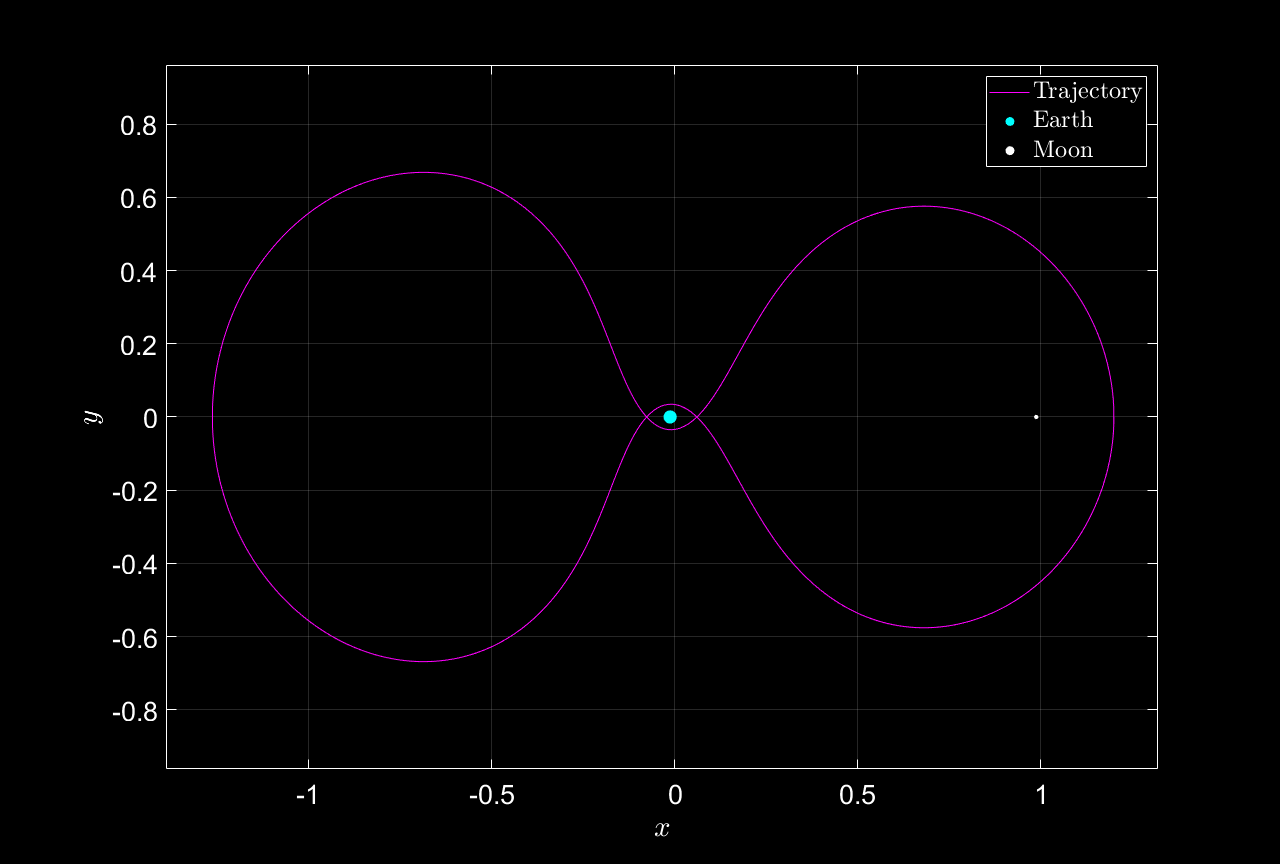
\includegraphics[width=\textwidth]{fig/trajectory1.png}
    \caption{Spacecraft Trajectory about the Earth \& Moon in the Synodic Frame}
    \label{fig1}
\end{figure}

\pagebreak

\begin{figure}[!h]
    \centering
    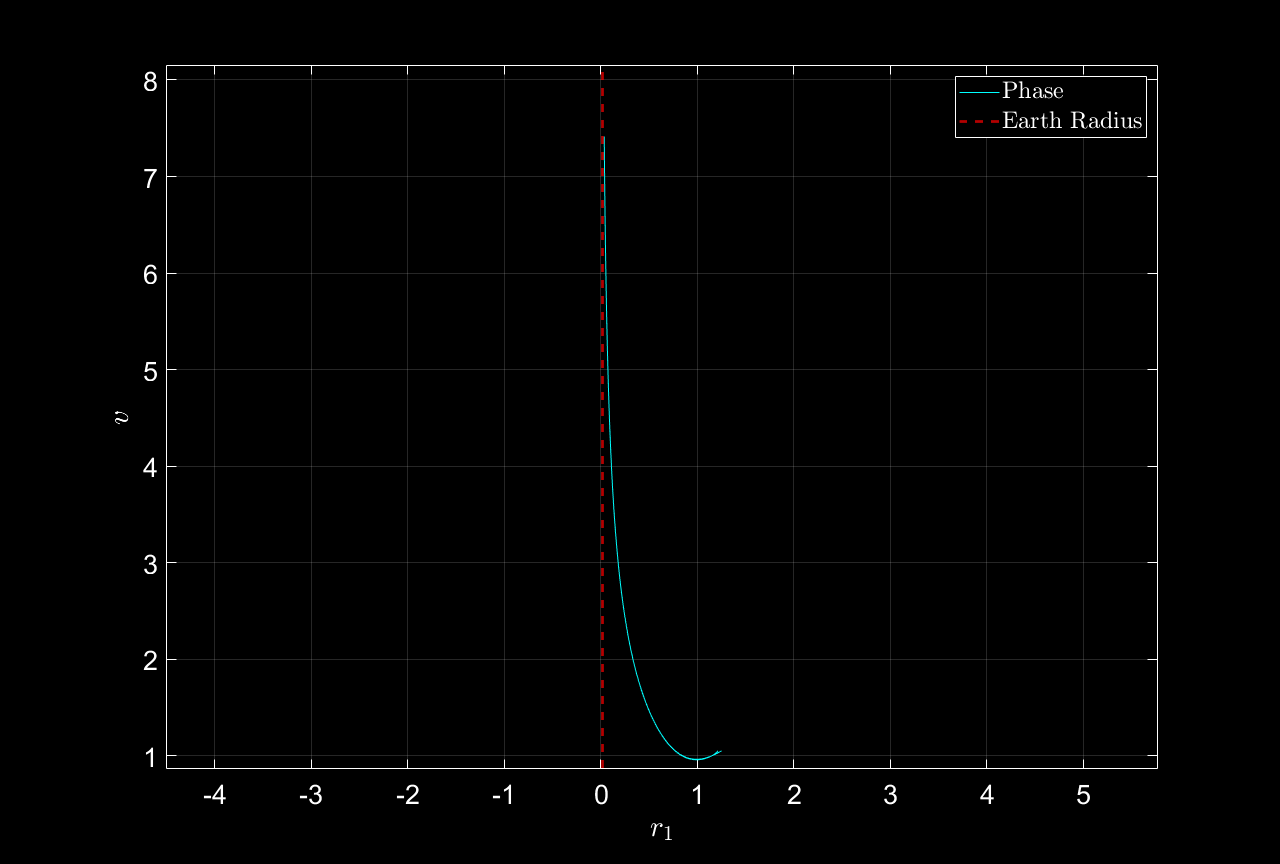
\includegraphics[width=\textwidth]{fig/phase1.png}
    \caption{Phase Space, \textit{Speed vs. Radial Distance from Earth}}
    \label{fig2}
\end{figure}


\begin{table}[h]
    \centering
    \caption{\cw Effects of Increasing the Number of Steps}
    \begin{tabular}{cccc} \toprule
        {$N$} & {$\mathrm{d}t$}    & {$r_1$}  & {$\mathrm{Test \ Criterion}$}                 \\ \midrule
        1000  & 0.0150             & 14.7302  & N/A                                           \\
        2000  & 0.0075             & 212.1128 & 0.9306                                        \\
        4000  & 0.0038             & 7.0135   & 29.2437                                       \\
        8000  & 0.0019             & 1.2056   & 4.8173                                        \\
        16000 & $\SI{9.3750E-4}{}$ & 1.1816   & 0.0203                                        \\
        32000 & $\SI{4.6875e-4}{}$ & 1.1808   & \color{magenta}$\SI{6.3125e-4}{}$ \cw $<$ tol \\ \bottomrule
    \end{tabular}
    \label{tab:table1}
\end{table}



\pagebreak

\subsection*{\underline{Scenario 2:}}

Initial Conditions:
\begin{multicols}{4}
    \begin{itemize}
        \item $x(0)$ = 1.2
        \item $y(0)$ = 0
        \item $v_x(0)$ = 0
        \item $f_d$ = 1
        \item $v_y(0)$ = -1.0493571
    \end{itemize}
\end{multicols}

\textbf{Note}: All quantities are in normalized units.

\vspace{\baselineskip}

These initial conditions are identical to the ones from the Scenario 1, but we set $f_d$ = 1, which corresponds to rockets firing in the retrograde direction with constant thrust through the entire flight. The trajectory will be calculated from $t$ = 0 to 4 normalized time units.

\vspace{\baselineskip}

The results are shown below:

\begin{figure}[h]
    \centering
    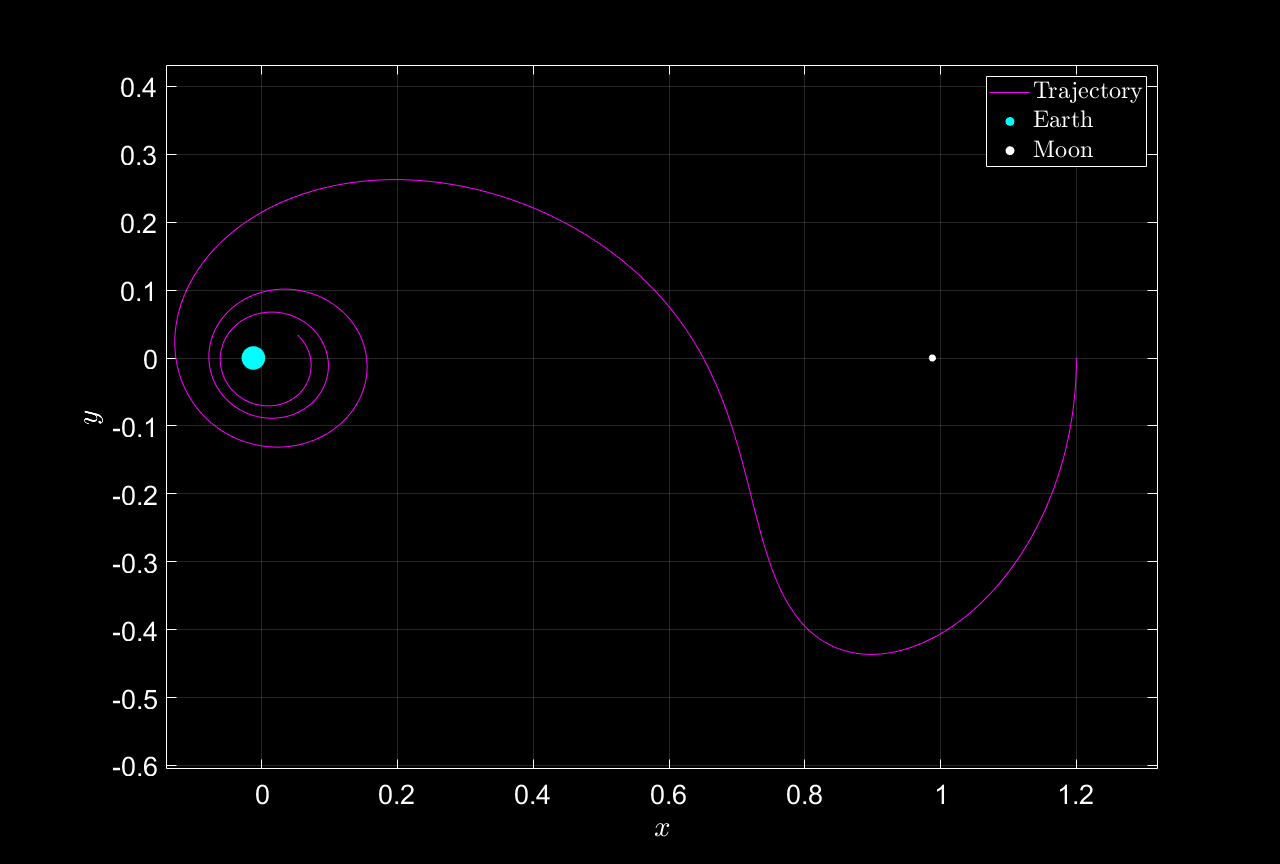
\includegraphics[width=\textwidth]{fig/trajectory2.png}
    \caption{Spacecraft Trajectory about the Earth \& Moon in the Synodic Frame}
    \label{fig3}
\end{figure}

\pagebreak

\begin{figure}[!h]
    \centering
    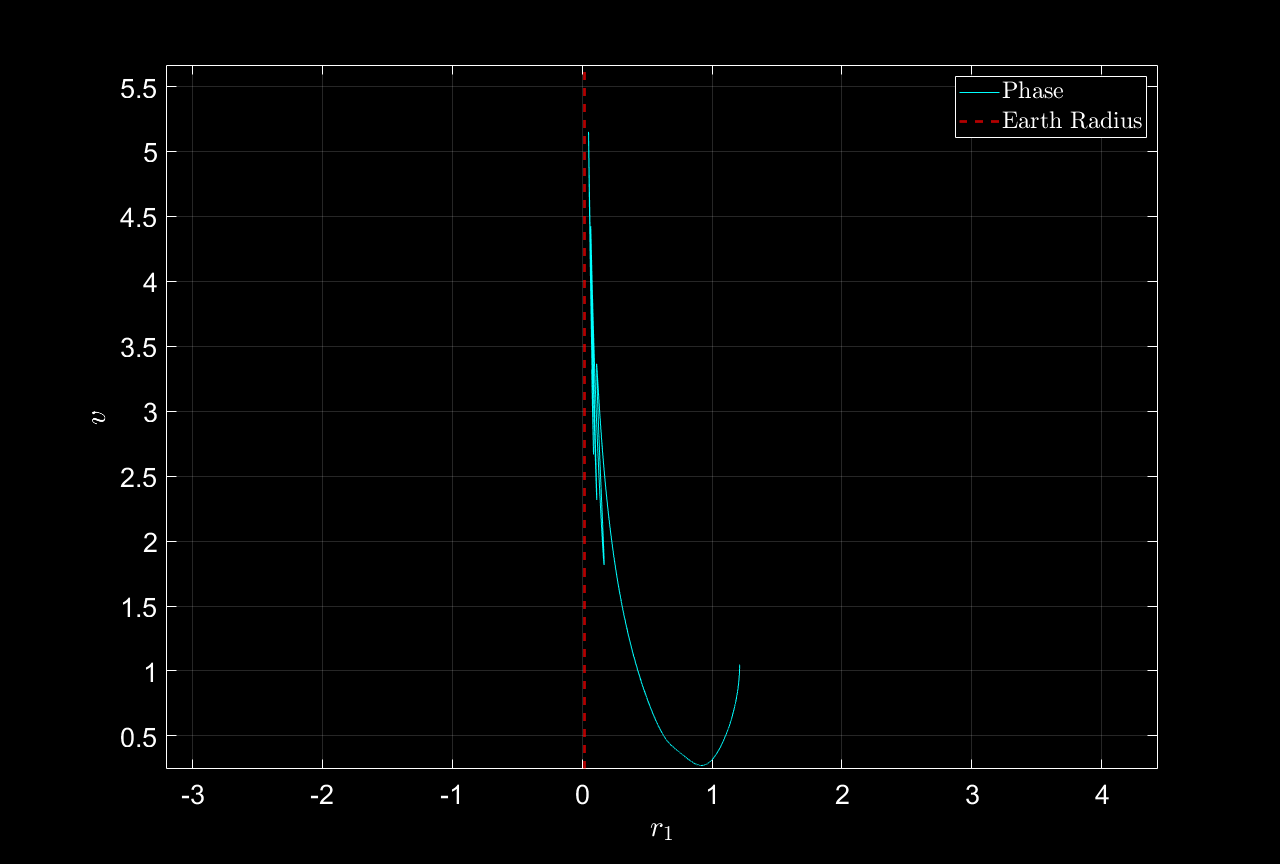
\includegraphics[width=\textwidth]{fig/phase2.png}
    \caption{Phase Space, \textit{Speed vs. Radial Distance from Earth}}
    \label{fig4}
\end{figure}


\begin{table}[h]
    \centering
    \caption{\cw Effects of Increasing the Number of Steps}
    \begin{tabular}{cccc} \toprule
        {$N$} & {$\mathrm{d}t$} & {$r_1$} & {$\mathrm{Test \ Criterion}$}      \\ \midrule
        1000  & 0.0040          & 0.0767  & N/A                                \\
        2000  & 0.0020          & 0.0748  & 0.0249                             \\
        4000  & 0.0010          & 0.0738  & 0.0144                             \\
        8000  & 0.0005          & 0.0732  & \color{magenta} 0.0075 \cw $<$ tol \\ \bottomrule
    \end{tabular}
    \label{tab:table2}
\end{table}